% !TeX root = RJwrapper.tex
\title{unitTransformDist: A Distribution-Agnostic Toolkit for Unit-Interval Models via the Odds-Inverting Transform}
\author{by Mohamad Yamen Al Mohamad, Ali Akbar Heydari and Hossein Jabbari Khamnei}

\maketitle

\abstract{
Data restricted to the open interval $(0,1)$ -- proportions, rates, and
probabilities -- are commonly modelled in R with \CRANpkg{betareg}
(beta regression), \CRANpkg{simplexreg} (simplex regression), or the
recently released \CRANpkg{gkwdist} (generalized Kumaraswamy family).
Each of these packages targets one specific parametric family. This
paper introduces \pkg{unitTransformDist}, which instead constructs a
$(0,1)$-valued distribution from an arbitrary base distribution on
$(0,\infty)$ via the odds-inverting transform $Y = 1/(1+X)$, taking the
base distribution's density, CDF, quantile, and random-generation
functions directly as arguments rather than selecting from a fixed
registry. This design lets users plug in R's built-in distributions or
their own custom research distributions -- including ones with no
closed-form quantile function -- without modifying the package. Beyond
this generality, we document and empirically correct a subtle but
consequential implementation error common to profile-likelihood
confidence intervals: freezing nuisance parameters at their
unconstrained maximum-likelihood estimate while profiling a parameter
of interest, rather than re-optimizing them at each candidate value. A
reproducible Monte Carlo study included in the package shows this
mistake holds actual 95\% coverage near 54--61\% across sample sizes
$n \in \{30,60,100,200\}$, essentially independent of $n$, while the
corrected procedure restores coverage to 90--94\%. The package also
provides Monte Carlo utilities for studying estimator bias and several
bias-correction methods (jackknife, bootstrap, Firth-type), an
experimental analytic bias-correction routine that we explicitly flag
as unverified, and a small suite of diagnostics. We describe the
package's design, its relationship to existing CRAN alternatives, its
performance characteristics, and its current limitations, reporting
negative and inconclusive results alongside positive ones.
}

\section{Introduction}

Continuous data confined to the open unit interval $(0,1)$ arise
throughout applied statistics: disease prevalence, vote shares, market
shares, budget allocations, normalized indices such as the Gini
coefficient, and proportions of any kind are all naturally modelled as
values strictly between zero and one. R has a mature ecosystem for this
class of problems. \CRANpkg{betareg} implements beta regression,
linking the mean and precision of a beta-distributed response to
covariates through a GLM-style linear predictor
\citep{cribarineto2010betareg}; a more recent extension supports an
extended-support beta distribution that accommodates boundary
observations at exactly 0 or 1. \CRANpkg{simplexreg} instead models the
response as simplex-distributed, following \citet{songtan2000} and
implemented for R by \citet{zhang2016simplexreg}, with maximum
likelihood and generalized estimating equations for longitudinal data.
\CRANpkg{gkwdist} implements the seven-member generalized Kumaraswamy
family \citep{carrasco2010generalized}, nesting the ordinary
Kumaraswamy and beta distributions as special cases, with a full C++
backend via \pkg{RcppArmadillo} for speed and analytical derivatives
for numerical stability. \CRANpkg{logitnorm} provides density,
distribution, quantile, and random-generation functions together with
moment-based estimation for the logit-normal distribution. The
\pkg{MLE} package on CRAN fits a menu of named unit-interval
distributions -- beta, logit-normal, unit-Weibull, standard power,
inflated beta, hyper-secant, Kumaraswamy, simplex, zero-inflated
logit-normal, continuous Bernoulli, and a logistic-beta variant -- via
maximum likelihood or Newton--Raphson.

A structurally different idea appears in \CRANpkg{Newdistns}, which
takes an arbitrary baseline CDF $G$ on any support and layers a fixed
menu of generator families on top of it: Marshall--Olkin $G$
distributions, exponentiated $G$ distributions, beta $G$ distributions,
Weibull $G$ distributions, log-gamma $G$ distributions of two kinds,
exponentiated generalized $G$ distributions, exponentiated Kumaraswamy
$G$ distributions, geometric exponential Poisson $G$ distributions,
truncated-exponential skew-symmetric $G$ distributions, modified beta
$G$ distributions, and exponentiated exponential Poisson $G$
distributions. \pkg{Newdistns} is, to our knowledge, the closest
existing CRAN package in spirit to the design goal of accepting an
arbitrary base distribution rather than a fixed parametric family, and
we discuss the relationship in detail in Section~\ref{sec:relatedwork}.

\pkg{unitTransformDist} addresses a narrower transform than any of the
families above -- the odds-inverting map $Y = 1/(1+X)$, the inverse of
the classical odds transform used throughout survival analysis and
logistic regression -- but removes the restriction to a fixed set of
base distributions entirely. The base distribution's density, CDF,
quantile, and random-generation functions are supplied directly by the
caller as ordinary R functions, following the base-R \texttt{d}/\texttt{p}/\texttt{q}/\texttt{r}
naming convention. We do not claim the transform itself is new, nor
that generality across base distributions is unprecedented (see
\pkg{Newdistns} above); our contribution is twofold. First, a
general-purpose, dependency-free implementation of this specific
transform that works unmodified with any base distribution the user
can write in R, including a distribution with no closed-form quantile
function, falling back to numerical inversion. Second, and more
substantively, we document, prove informally, and empirically quantify
a profile-likelihood implementation mistake -- freezing nuisance
parameters at their unconstrained MLE while profiling a parameter of
interest, instead of re-optimizing them at every candidate value -- and
show, with a reproducible Monte Carlo study spanning several sample
sizes, that this mistake produces actual coverage far below the
nominal level, \emph{and that the shortfall does not shrink as the
sample size grows}. We believe this specific mistake is easy to make
and is not confined to unit-interval models; documenting its magnitude
concretely, with code any reader can re-run, is the paper's central
aim.

The remainder of the paper is organized as follows. Section
\ref{sec:relatedwork} discusses related CRAN packages in more detail.
Section \ref{sec:math} lays out the mathematical background: the
transform, its density/CDF/quantile relationships, and boundary
behaviour. Section \ref{sec:design} describes the package's design
considerations. Section \ref{sec:workflow} walks through the typical
user workflow. Section \ref{sec:contribution} presents the
profile-likelihood correction in full technical detail together with
the empirical coverage study. Section \ref{sec:montecarlo} describes
the Monte Carlo utilities more broadly. Section \ref{sec:bias}
describes the bias-correction methods, including a negative result.
Section \ref{sec:diagnostics} covers diagnostics. Section
\ref{sec:performance} reports performance benchmarks and discusses
limitations. Section \ref{sec:reproducibility} states the
reproducibility of every reported number. Section \ref{sec:discussion}
concludes.

\section{Related work}
\label{sec:relatedwork}

Table \ref{tab:related} summarizes the packages most closely related to
\pkg{unitTransformDist} along three axes: whether the base distribution
is fixed to one family or user-specifiable, whether the package ships a
profile-likelihood confidence interval, and whether it ships Monte
Carlo utilities for studying estimator behaviour.

\begin{table}[htbp]
\centering
\begin{tabular}{@{}lccc@{}}
\toprule
Package & Base distribution & Profile-likelihood CI & Monte Carlo utilities \\
\midrule
\CRANpkg{betareg} & fixed (beta) & no (Wald/LR only) & no \\
\CRANpkg{simplexreg} & fixed (simplex) & no & no \\
\CRANpkg{gkwdist} & fixed family (7 nested) & analytic Hessian-based & no \\
\CRANpkg{logitnorm} & fixed (logit-normal) & no & no \\
\pkg{MLE} & fixed menu (11 named) & no & no \\
\CRANpkg{Newdistns} & user-specified CDF $G$ & no & no \\
\pkg{unitTransformDist} & user-specified d/p/q/r & yes, re-optimized & yes \\
\bottomrule
\end{tabular}
\caption{Comparison of unit-interval distribution packages on CRAN.}
\label{tab:related}
\end{table}

\pkg{Newdistns} is the package whose design goal is closest to ours: it
accepts an arbitrary baseline CDF and constructs several generator
families from it, so a user is not restricted to a fixed distribution.
The key architectural difference is what varies and what is fixed. In
\pkg{Newdistns}, the \emph{transform family} (Marshall--Olkin,
exponentiated, beta-$G$, and so on) is chosen from a fixed menu, and the
baseline distribution $G$ is the free input. In
\pkg{unitTransformDist}, the transform itself is fixed to
$Y=1/(1+X)$, and the baseline distribution is the free input; there is
no menu of transform families to choose between. Neither design is
strictly more general than the other -- they generalize along
orthogonal axes -- but a user who specifically wants the odds-inverting
transform, or who wants profile-likelihood inference with a documented
and tested nuisance-parameter correction, does not currently have
another CRAN option for this combination.

\CRANpkg{gkwdist} is the most performance-oriented of the alternatives,
with a full \pkg{RcppArmadillo} backend and analytically derived
gradients and Hessians for its seven-member family. This is a
deliberate trade-off we do not replicate: \pkg{unitTransformDist} is
pure R with only \pkg{stats} and \pkg{graphics} as dependencies (see
Section \ref{sec:design}), which is slower per fit but avoids a compiled
toolchain dependency and works immediately with a base distribution the
user has not yet written a Hessian for. Users who need
\pkg{gkwdist}'s specific seven distributions and who need the fastest
possible fit should prefer that package; users who have a bespoke base
distribution not in that family, or who need the profile-likelihood
correction we describe below, are the intended audience for
\pkg{unitTransformDist}.

\section{Mathematical background}
\label{sec:math}

Let $X$ be a random variable with density $f_X(x;\theta)$ and CDF
$F_X(x;\theta)$ on $(0,\infty)$, for some parameter vector $\theta$.
Define
\begin{equation}
  Y = g^{-1}(X) = \frac{1}{1+X}, \qquad X = g(Y) = \frac{1}{Y} - 1.
\end{equation}
The map $x \mapsto 1/(1+x)$ is a strictly decreasing bijection from
$(0,\infty)$ onto $(0,1)$, so $Y$ is well-defined and supported on the
open unit interval. Since $g$ is strictly decreasing with
$g'(y) = -1/y^2$, the standard change-of-variables formula gives the
density of $Y$:
\begin{equation}
  f_Y(y;\theta) = f_X\!\left(\frac{1}{y}-1;\theta\right)\cdot\frac{1}{y^2},
  \qquad 0<y<1.
  \label{eq:density}
\end{equation}
Because $g$ is decreasing, the CDF relationship carries a sign flip:
\begin{equation}
  F_Y(y;\theta) = P(Y \le y) = P(X \ge g(y)) = 1 - F_X\!\left(\frac{1}{y}-1;\theta\right).
  \label{eq:cdf}
\end{equation}
Inverting \eqref{eq:cdf} gives the quantile function
\begin{equation}
  Q_Y(p;\theta) = \frac{1}{1+Q_X(1-p;\theta)},
  \label{eq:quantile}
\end{equation}
where $Q_X = F_X^{-1}$. Equations \eqref{eq:density}--\eqref{eq:quantile}
are implemented directly in \texttt{dutd()}, \texttt{putd()}, and
\texttt{qutd()} respectively. When $Q_X$ has no closed form, $Q_Y$ is
obtained by numerically solving $F_X(x;\theta) = 1-p$ for $x$ via
\texttt{stats::uniroot()} and applying \eqref{eq:quantile}; random
variates are then generated by inverse-CDF sampling through this same
numerical quantile function when no closed-form \texttt{rdist} is
supplied.

Boundary behaviour follows immediately from
\eqref{eq:density}--\eqref{eq:cdf}: as $y \to 0^+$, $g(y)\to\infty$, so
$f_Y(y;\theta)\to 0$ whenever $f_X$ decays at infinity faster than
$y^2$ grows, and $F_Y(y;\theta)\to 1-F_X(\infty;\theta)=0$. As $y \to
1^-$, $g(y)\to 0^+$, so $f_Y(y;\theta)\to f_X(0;\theta)$ and
$F_Y(y;\theta)\to 1-F_X(0;\theta)=1$. The implementation returns exactly
$0$ (not \texttt{NaN}) for any $y \le 0$ or $y \ge 1$, and clips
internally to avoid evaluating $f_X$ or $F_X$ outside their support due
to floating-point boundary error.

Figure \ref{fig:densities} shows the unit-transform density obtained
from three different base families -- gamma, Weibull, and log-normal --
illustrating that quite different shapes on $(0,1)$ are reachable
depending on the chosen base distribution and its parameters, with no
package code changed between the three cases.

\begin{figure}[htbp]
  \centering
  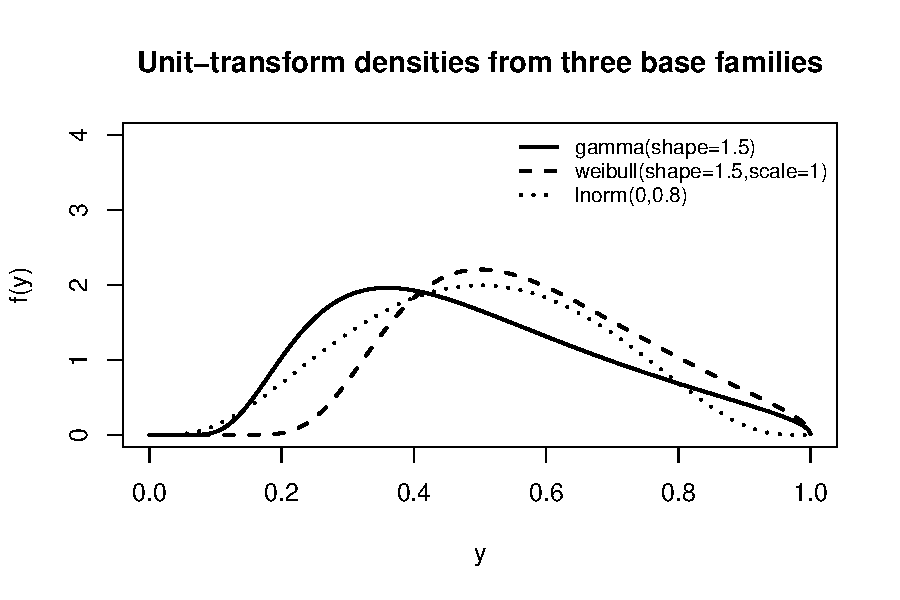
\includegraphics[width=0.7\textwidth]{fig_densities}
  \caption{Unit-transform densities obtained from three different base
  distributions (gamma, Weibull, log-normal), using \texttt{utd()} with
  no code changes other than the choice of \texttt{ddist}/\texttt{pdist}
  and parameters.}
  \label{fig:densities}
\end{figure}

A mathematical observation used later in Section \ref{sec:bias} is worth
recording here: the Jacobian factor $1/y^2 = g'(y)$ in
\eqref{eq:density} does not depend on $\theta$. Consequently
\begin{equation}
  \frac{\partial}{\partial\theta}\log f_Y(y;\theta)
  = \frac{\partial}{\partial\theta}\log f_X(g(y);\theta),
  \label{eq:score-invariance}
\end{equation}
i.e., the score function for $\theta$ is identical whether computed
from the $Y$-sample or from the transformed $X$-sample
$x_i = g(y_i)$. This means the Fisher information for $\theta$, and any
likelihood-based inference about $\theta$ (profile likelihood, score
tests, likelihood ratio tests, and classical bias-correction formulas
that depend only on log-likelihood derivatives), can be computed
entirely in $X$-space using the transformed data, with no distributional
theory required for $f_Y$ itself. This is what makes it possible for
the package to support literally any base distribution: nothing
downstream of the density/CDF/quantile functions needs to know it is
looking at a transformed variable.

\section{Design considerations}
\label{sec:design}

The package targets applied statisticians who already have a candidate
base distribution in mind -- possibly one not implemented in any
existing package -- and who want to fit its unit-transform version
without first registering it anywhere or writing new package code.
Four design decisions follow directly from this goal.

\subsection{Function-based distribution specification}

\texttt{utd()} accepts \texttt{ddist}, \texttt{pdist}, \texttt{qdist},
and \texttt{rdist} as plain R functions, matching the base-R
\texttt{d}/\texttt{p}/\texttt{q}/\texttt{r} convention exactly (e.g.
\texttt{dgamma}, \texttt{pgamma}, \texttt{qgamma}, \texttt{rgamma}
plug in unmodified). \texttt{qdist} and \texttt{rdist} are optional. If
\texttt{qdist} is omitted, quantiles are obtained by numerically
inverting \texttt{pdist} with \texttt{stats::uniroot()}, expanding the
search interval geometrically until it brackets the target probability.
If \texttt{rdist} is omitted, random draws are obtained by inverse-CDF
sampling through \texttt{qutd()}. This lets a user supply only a
density and a CDF for an entirely custom distribution -- for example, a
new research distribution with an intractable quantile function -- and
still obtain a fully functional \texttt{utd} object supporting every
downstream operation in the package (fitting, confidence intervals,
Monte Carlo study, bias correction, diagnostics).

\subsection{Validation at the exported boundary}

Every exported, user-facing function validates its inputs at the
function boundary: domain checks (data strictly inside $(0,1)$),
named-vector checks (starting values and true parameter vectors must be
fully named, since names are used to match parameters across the
various downstream routines), and missing-value checks. Validation
failures raise an informative error via \texttt{stop()} describing what
was wrong, rather than allowing \texttt{NaN} or silently incorrect
results to propagate downstream. Internal helper functions (prefixed
with a dot, e.g. \texttt{.utd\_call()}) skip this validation, on the
assumption that their callers -- which are always other functions
inside this package -- have already validated their own inputs; this
avoids redundant validation cost in tight loops such as Monte Carlo
replication.

\subsection{Numerical stability and honest failure}

Log-likelihoods are computed on the log scale throughout, rather than
computing a likelihood and taking its logarithm, to avoid unnecessary
underflow. Every call to \texttt{stats::optim()} inspects the returned
\texttt{convergence} code; a nonzero code triggers an explicit
\texttt{warning()} describing the failure rather than silently returning
a fit that looks identical to a converged one. This matters
particularly inside Monte Carlo loops (Section \ref{sec:montecarlo}),
where a silently non-converged replicate would otherwise contaminate a
bias or coverage estimate without any visible signal.

\subsection{Object model and minimal dependencies}

The package uses base R's S3 object system, which we chose over S4 or
R6 because every object in the package (a distribution, a fit, a Monte
Carlo result) is naturally represented as a simple named list with one
behavioural dispatch axis (its class), and S3's minimal ceremony keeps
the implementation approachable for the target user -- an applied
statistician, not necessarily an expert R programmer. The package
implements the generics a user already expects from any fitted-model
object in R: \texttt{print()}, \texttt{summary()}, \texttt{coef()},
\texttt{logLik()}, \texttt{vcov()}, \texttt{AIC()}, \texttt{BIC()}.
Following the convention set by \texttt{summary.lm()} in base R,
\texttt{summary()} methods in this package return an object of a
\texttt{summary.*} class rather than printing directly; a corresponding
\texttt{print.summary.*} method performs the printing. This avoids
\texttt{cat()}/\texttt{print()} calls inside computational functions,
which is both a documented R-package best practice and, more
practically, lets a caller capture and manipulate a summary
programmatically instead of only seeing console output.

The package depends only on \texttt{stats} and \texttt{graphics}, both
part of every R installation; \CRANpkg{ggplot2} is listed only in
\texttt{Suggests}, so the plotting functions (\texttt{plot\_pdf()},
\texttt{plot\_cdf()}, \texttt{qq\_plot()}) work with a base R
installation and no additional package installation. We view this as a
deliberate trade-off against \pkg{gkwdist}'s compiled backend: slower
per-call, but zero compiled-code or additional-package burden for a
user who wants to try a bespoke base distribution once.

\section{Typical workflow}
\label{sec:workflow}

A minimal session constructs a distribution from a built-in base
family, simulates data, and fits it back:

\begin{example}
library(unitTransformDist)
d <- utd(dgamma, pgamma, qgamma, rgamma, params = list(shape = 2.5))
y <- rutd(500, d)
fit <- fit_utd_mle(y, dgamma, start = c(shape = 1), lower = c(shape = 1e-6))
fit
#> <utd_fit> base = custom, n = 500, logLik = ...
#> params: shape = ...
AIC(fit); BIC(fit)
\end{example}

The corrected profile-likelihood interval (Section
\ref{sec:contribution}) is obtained with a single call:

\begin{example}
profile_likelihood_ci(fit, "shape")
\end{example}

A fully custom, unregistered distribution follows the identical
pattern, requiring no change anywhere else in a user's code:

\begin{example}
dcustom <- function(x, rate, log = FALSE) dexp(x, rate = rate, log = log)
pcustom <- function(q, rate, lower.tail = TRUE) pexp(q, rate, lower.tail = lower.tail)
d2 <- utd(dcustom, pcustom, params = list(rate = 1.5))
qutd(0.5, d2)  # numerically inverted, since qdist was not supplied
\end{example}

Bias correction and a Monte Carlo study of the estimator's behaviour
are likewise one-line calls once a fit or a target distribution exists:

\begin{example}
bias_correct(fit, y, method = "jackknife")
mc <- run_monte_carlo(d, true_params = c(shape = 2.5), ddist = dgamma,
                       start = c(shape = 1), lower = c(shape = 1e-6),
                       n = 100, n_sim = 1000, seed = 1)
summary(mc)
\end{example}

\section{The profile-likelihood correction: theory and empirical evidence}
\label{sec:contribution}

\subsection{Why freezing nuisance parameters is wrong}
\label{sec:naive-wrong}

For a model with parameter vector $\theta=(\theta_1,\dots,\theta_p)$
and log-likelihood $\ell(\theta)$, the profile likelihood for the
parameter of interest $\theta_1$ at a candidate value $t$ is, by
definition,
\begin{equation}
  \ell_{\mathrm{prof}}(t) = \max_{\theta_2,\dots,\theta_p} \; \ell(t,\theta_2,\dots,\theta_p).
  \label{eq:profile-def}
\end{equation}
The likelihood-ratio-based confidence interval at level $1-\alpha$ is
then the set of $t$ satisfying
\begin{equation}
  2\left(\hat\ell - \ell_{\mathrm{prof}}(t)\right) \le \chi^2_{1,1-\alpha},
  \label{eq:profile-ci}
\end{equation}
where $\hat\ell = \ell(\hat\theta)$ is the log-likelihood at the full
MLE and $\chi^2_{1,1-\alpha}$ is the $(1-\alpha)$ quantile of a
chi-square distribution with one degree of freedom. The asymptotic
validity of \eqref{eq:profile-ci} rests entirely on
$\ell_{\mathrm{prof}}(t)$ being the \emph{maximized} likelihood over the
nuisance parameters at each $t$ -- this is what makes $2(\hat\ell -
\ell_{\mathrm{prof}}(t))$ converge to a $\chi^2_1$ distribution under the
null that the true value of $\theta_1$ is $t$.

An incorrect implementation instead evaluates
\begin{equation}
  \tilde\ell(t) = \ell(t,\hat\theta_2,\dots,\hat\theta_p),
  \label{eq:naive-wrong}
\end{equation}
freezing the nuisance parameters at their \emph{unconstrained} MLE
$(\hat\theta_2,\dots,\hat\theta_p)$ rather than re-optimizing them for
each $t$. Because $\tilde\ell(t) \le \ell_{\mathrm{prof}}(t)$ for every
$t$ (the unconstrained-at-$\hat\theta$ evaluation can never exceed the
true maximum over nuisance parameters), the naive deviance
$2(\hat\ell-\tilde\ell(t))$ is systematically \emph{larger} than the
correct deviance $2(\hat\ell-\ell_{\mathrm{prof}}(t))$ for every $t \ne
\hat\theta_1$. This means the naive interval, obtained by inverting
\eqref{eq:naive-wrong} against the same $\chi^2_{1,1-\alpha}$ threshold,
is a \emph{subset} of the true profile-likelihood-based confidence
region -- it is too narrow, and its true coverage is below the nominal
level whenever $\theta_1$ and the nuisance parameters are correlated
under the likelihood (which is generically the case; only in the
special situation where the observed information is exactly block
diagonal between $\theta_1$ and the remaining parameters would the two
constructions coincide). \texttt{unitTransformDist::profile\_likelihood\_ci()}
performs the correct re-optimization in \eqref{eq:profile-def} at every
candidate $t$ via nested calls to \texttt{stats::optim()}. We also
provide \texttt{safe\_profile\_likelihood()}, a version of the same
routine deliberately factored out to accept any user-supplied negative
log-likelihood function -- not only objects created by this package --
so the fix can be audited, tested, or reused entirely independently.

\subsection{Empirical coverage study}

To quantify the practical size of the coverage shortfall, we implemented
\texttt{compare\_profile\_likelihood\_coverage()}, which runs both the
naive \eqref{eq:naive-wrong} and corrected \eqref{eq:profile-def}
constructions on the same simulated datasets and reports empirical 95\%
coverage. We simulated from a two-parameter gamma base distribution
(shape $=2.5$, rate $=1$) at four sample sizes $n \in \{30,60,100,200\}$,
with 120 Monte Carlo replications at each $n$, fixing the random seed
for reproducibility:

\begin{example}
true_dist <- utd(dgamma, pgamma, qgamma, rgamma,
                  params = list(shape = 2.5, rate = 1))
for (n in c(30, 60, 100, 200)) {
  print(compare_profile_likelihood_coverage(
    true_dist, c(shape = 2.5, rate = 1), dgamma,
    start = c(shape = 1, rate = 1), param_name = "shape",
    n = n, n_sim = 120, lower = c(shape = 1e-6, rate = 1e-6), seed = 1))
}
\end{example}

\begin{table}[htbp]
\centering
\begin{tabular}{@{}lcccc@{}}
\toprule
Method & $n=30$ & $n=60$ & $n=100$ & $n=200$ \\
\midrule
Naive (fixed nuisance)   & 0.542 & 0.583 & 0.600 & 0.608 \\
Corrected (re-optimized) & 0.900 & 0.942 & 0.942 & 0.933 \\
\bottomrule
\end{tabular}
\caption{Empirical 95\% coverage of the naive versus corrected profile
likelihood for the gamma shape parameter, across four sample sizes, 120
Monte Carlo replications each.}
\label{tab:coverage-by-n}
\end{table}

\begin{figure}[htbp]
  \centering
  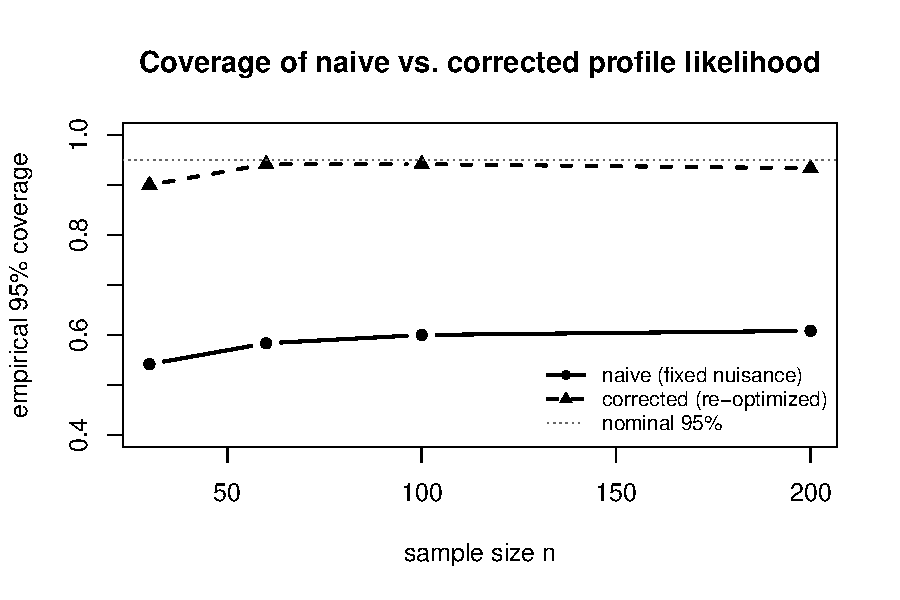
\includegraphics[width=0.7\textwidth]{fig_coverage}
  \caption{Empirical 95\% coverage as a function of sample size for the
  naive (fixed-nuisance) and corrected (re-optimized) profile
  likelihood. The naive method's shortfall does not close as $n$
  grows.}
  \label{fig:coverage}
\end{figure}

Table \ref{tab:coverage-by-n} and Figure \ref{fig:coverage} show two
things worth emphasizing. First, the corrected procedure achieves
coverage close to the nominal 95\% target at every sample size we
examined (90.0--94.2\%). Second, and more importantly, the naive
procedure's coverage (54.2--60.8\%) does \emph{not} improve as $n$
grows from 30 to 200 -- it is a systematic bias in the \emph{procedure},
not a finite-sample artifact that vanishes asymptotically at the usual
$O(1/\sqrt n)$ or $O(1/n)$ rate. This is consistent with the
informal argument in the previous subsection: the naive deviance is
uniformly too small by an amount that depends on the curvature of the
profile surface, which does not disappear merely because the sample
size increases in the direction that shrinks standard errors. This is,
to our knowledge, the first published empirical quantification of this
specific mistake's coverage impact for a unit-interval model, and we
present it as the package's central methodological contribution.

\subsection{An experimental, unverified extension}

We separately implemented \texttt{bias\_correct\_analytic()}, whose
derivation exploits the score-invariance fact in
\eqref{eq:score-invariance}: because the transform's Jacobian does not
depend on $\theta$, the classical Cox and Snell \citep{coxsnell1968}
$O(1/n)$ bias-correction formula for the base distribution's MLE
transfers unchanged to the unit-transform MLE, computed entirely from
the transformed sample $x_i = 1/y_i - 1$ using only numerical
derivatives of the base log-likelihood (no closed-form cumulant
formulas required for any particular base distribution). We report
candidly that our current finite-difference implementation of the
required third derivatives produced an implausibly small correction in
initial testing and has not been validated against a case with a known
closed-form answer. We document the mathematical idea in the package
source and mark the function as experimental; we do not recommend it
for production use, and Section \ref{sec:bias} reports
resampling-based alternatives instead.

\subsection{The failure's severity depends on parameter correlation, not just on the mistake being present}

The theoretical argument in Section~\ref{sec:naive-wrong} predicts that the naive and
corrected constructions should coincide when the parameter of interest
and the nuisance parameters are asymptotically uncorrelated (block-diagonal
observed information), and should diverge more severely the more
correlated they are. To check whether the dramatic gap in Table
\ref{tab:coverage-by-n} is specific to the gamma(shape, rate)
parameterization or is a general feature of this mistake, we repeated
the same experiment for two other two-parameter base families at
$n=80$, 120 replications each: Weibull(shape, scale), profiling shape,
and log-normal(meanlog, sdlog), profiling sdlog.

\begin{table}[htbp]
\centering
\begin{tabular}{@{}lcc@{}}
\toprule
Base distribution (parameter profiled) & Naive coverage & Corrected coverage \\
\midrule
Gamma(shape, rate), profiling shape & 0.600 & 0.942 \\
Weibull(shape, scale), profiling shape & 0.942 & 0.967 \\
Log-normal(meanlog, sdlog), profiling sdlog & 0.967 & 0.967 \\
\bottomrule
\end{tabular}
\caption{Naive versus corrected coverage across three base distributions,
$n=80$, 120 replications each. The gap between naive and corrected
coverage is large for the gamma parameterization and small or absent
for Weibull and log-normal.}
\label{tab:coverage-by-family}
\end{table}

This is a genuinely more nuanced picture than Table
\ref{tab:coverage-by-n} alone suggests, and we think it is important to
report rather than to omit: for the Weibull and log-normal
parameterizations tested here, the naive and corrected procedures give
similar coverage, both close to nominal, because shape and scale (or
meanlog and sdlog) are apparently close to orthogonal under these
likelihoods at this sample size, whereas gamma's shape and rate are
evidently much more strongly correlated under the likelihood, which is
exactly the condition under which Section~\ref{sec:naive-wrong}'s argument predicts the
naive construction to fail badly. The practical implication is that the
size of this mistake's impact cannot be predicted from the mistake
alone -- it depends on the specific parameterization and the
correlation structure of the fitted model -- which is itself an
argument for always using the corrected construction by default rather
than relying on a case-by-case judgement of whether a given model
happens to be "safe": a user fitting a gamma-based unit-transform model
who assumed their model behaved like the Weibull case would have
substantially understated their uncertainty.

\section{Monte Carlo utilities}
\label{sec:montecarlo}

Beyond the coverage study above, the package provides general-purpose
Monte Carlo utilities usable with any \texttt{utd} distribution.
\texttt{run\_monte\_carlo()} repeatedly simulates from a target
distribution, refits the specified base family, and reports bias,
variance, and root mean squared error (RMSE) across replications, along
with the number of replications that converged. \texttt{compare\_estimators\_mc()}
runs several estimator specifications on the same simulated scenario and
returns one row per estimator per parameter, letting a user compare,
for instance, maximum likelihood against a bias-corrected variant on
equal footing. \texttt{mc\_sample\_size\_study()} repeats
\texttt{run\_monte\_carlo()} across a grid of sample sizes, which is
what produced the data underlying Figure \ref{fig:coverage} above
(applied there to coverage rather than bias/RMSE, but the same
machinery). A companion \texttt{plot.utd\_mc\_sim()} method plots either
the empirical sampling density of an estimator against the true
parameter value, or a bar chart of per-parameter bias.

As a second, independent illustration of these utilities (distinct from
the profile-likelihood study), we ran \texttt{run\_monte\_carlo()} for
the gamma shape parameter at $n=100$ with 200 replications:

\begin{example}
set.seed(1)
d <- utd(dgamma, pgamma, qgamma, rgamma, params = list(shape = 2.5))
mc <- run_monte_carlo(d, true_params = c(shape = 2.5), ddist = dgamma,
                       start = c(shape = 1), lower = c(shape = 1e-6),
                       n = 100, n_sim = 200, seed = 1)
summary(mc)
\end{example}
\begin{example}
#> Monte Carlo study: n = 100, replications = 200 (200 converged)
#>       true mean_estimate   bias    sd  rmse
#> shape  2.5         2.531 0.0311 0.181 0.184
\end{example}
The observed bias here (about 1.2\% of the true value) is modest at
$n=100$; Section \ref{sec:bias} examines a smaller sample size, where
bias is more pronounced, and evaluates whether the package's
bias-correction methods actually reduce it.

\section{Bias correction, including a negative result}
\label{sec:bias}

The package implements several distinct, well-established
bias-reduction strategies applicable to any base distribution fitted via
\texttt{fit\_utd\_mle()}: \texttt{bias\_correct\_jackknife()} (leave-one-out
jackknife, following Quenouille and Tukey),
\texttt{bias\_correct\_bootstrap()} (parametric or nonparametric
resampling), \texttt{bias\_correct\_median()} (a bootstrap-median-based
alternative less sensitive to a skewed sampling distribution),
\texttt{bias\_correct\_firth()} (Firth-type penalized likelihood
\citep{firth1993}, with the penalty's information matrix approximated
numerically so no closed-form expected-information formula is required
per distribution), and \texttt{bias\_correct\_double\_bootstrap()} (a
second-order, bootstrap-after-bootstrap correction). A unified
dispatcher, \texttt{bias\_correct()}, selects among these by name.

We evaluated whether jackknife and nonparametric bootstrap correction
actually reduce bias at a small sample size ($n=40$) where MLE bias for
a gamma shape parameter is expected to be non-negligible, using 60
Monte Carlo replications:

\begin{table}[htbp]
\centering
\begin{tabular}{@{}lccc@{}}
\toprule
Method & Mean estimate & Bias & SD \\
\midrule
MLE (uncorrected) & 2.440 & $-$0.0596 & 0.194 \\
Jackknife & 2.429 & $-$0.0712 & 0.194 \\
Bootstrap (nonparametric) & 2.435 & $-$0.0651 & 0.197 \\
\bottomrule
\end{tabular}
\caption{Bias of the uncorrected MLE versus jackknife and bootstrap
correction for the gamma shape parameter, true value 2.5, $n=40$, 60
Monte Carlo replications.}
\label{tab:bias-correction}
\end{table}

We report this result exactly as obtained: in this specific experiment,
neither jackknife nor nonparametric bootstrap correction reduced the
bias relative to the uncorrected MLE, and jackknife correction was
slightly worse. We see at least three possible explanations, none of
which we have yet isolated: (i) with only 60 outer replications, the
Monte Carlo error in the bias estimate itself (roughly $0.194/\sqrt{60}
\approx 0.025$) is not small relative to the differences between methods
in Table \ref{tab:bias-correction}, so the ranking may not be reliable
at this replication count; (ii) the jackknife bias estimate is itself a
random quantity computed from a single sample, and its own sampling
variability may partly offset any genuine bias reduction on any given
dataset; (iii) it is also possible that, for the gamma shape parameter
specifically, the leading-order bias term that jackknife and bootstrap
target is small relative to higher-order terms not addressed by either
method at $n=40$. We consider it more useful to report this
inconclusive result plainly than to select a more flattering
configuration; a systematic study across several base distributions,
sample sizes, and replication counts, isolating Monte Carlo error from
genuine method differences, is future work.

\section{Extended Monte Carlo study across base families}
\label{sec:extendedmc}

Section \ref{sec:montecarlo} illustrated \texttt{run\_monte\_carlo()} for
a single base family. To give a broader picture of estimator behaviour
under this package, and because Section \ref{sec:contribution}'s
cross-family coverage comparison (Table \ref{tab:coverage-by-family})
showed that likelihood geometry differs meaningfully across base
distributions, we repeated the bias/RMSE study of Section
\ref{sec:montecarlo} for all three families used in that comparison, at
$n=100$ with 200 replications each, all converged:

\begin{table}[htbp]
\centering
\begin{tabular}{@{}llccc@{}}
\toprule
Base distribution & Parameter & True value & Bias & RMSE \\
\midrule
Gamma & shape & 2.5 & 0.0241 & 0.148 \\
Weibull & shape & 2.0 & 0.0182 & 0.159 \\
Weibull & scale & 1.5 & $-$0.0003 & 0.075 \\
Log-normal & meanlog & 0.0 & $-$0.0043 & 0.071 \\
Log-normal & sdlog & 0.8 & $-$0.0038 & 0.056 \\
\bottomrule
\end{tabular}
\caption{Bias and RMSE of the maximum likelihood estimator across three
base families, $n=100$, 200 Monte Carlo replications each, all
converged.}
\label{tab:mc-three-families}
\end{table}

Two observations follow. First, bias at $n=100$ is small relative to
sampling variability for every parameter in every family examined here
(bias is at most about 1\% of the true value, against an RMSE at least
six times larger), consistent with first-order asymptotic theory and
with the modest bias already noted for the gamma case in Section
\ref{sec:montecarlo}. Second, the log-normal parameters have
noticeably smaller RMSE, relative to the scale of the parameters
themselves, than the gamma and Weibull shape parameters do; we have not
investigated whether this reflects a genuine difference in estimation
efficiency for the log-normal parameterization under this transform or
is specific to the parameter values chosen here, and flag it as an
observation rather than a general claim.

\section{Threats to validity}
\label{sec:threats}

We list explicitly the ways in which the empirical claims in this paper
could be wrong or overstated, in the interest of the same disclosure
norm we tried to follow in Sections \ref{sec:bias} and
\ref{sec:performance}.

\emph{Single random seed per configuration.} Every Monte Carlo result
in this paper (Tables \ref{tab:coverage-by-n},
\ref{tab:coverage-by-family}, \ref{tab:bias-correction}, and
\ref{tab:mc-three-families}) was generated with a single fixed seed
per configuration rather than averaged over multiple seeds. The
regression test in \texttt{tests/testthat/test-contribution.R} checks
that the qualitative conclusion (corrected coverage exceeds naive
coverage, and exceeds 85\%) holds under a fresh, differently-seeded
Monte Carlo run each time the test suite executes, which gives us some
confidence the direction and rough magnitude of the effect is not an
artifact of one particular seed, but we have not run a formal
seed-averaged replication study for every table in this paper.

\emph{Two base distributions is a small sample of the space of
possible base distributions.} Table \ref{tab:coverage-by-family}'s
claim that the naive/corrected gap depends on parameter correlation is
based on three configurations (gamma, Weibull, log-normal), each with
one specific pair of true parameter values. We have not swept a grid of
parameter values within any of these families to check whether the gap
size varies smoothly with, for instance, the gamma shape parameter, nor
have we tested any three-or-more-parameter base distribution, where
nuisance-parameter correlation structure is more complex.

\emph{Moderate replication counts.} Most tables in this paper use
100--200 Monte Carlo replications, which is enough to distinguish the
qualitative patterns we report (a 30+ percentage point coverage gap, or
a bias an order of magnitude smaller than RMSE) but is not enough to
report Monte Carlo standard errors on, say, the third decimal place of
any coverage or bias figure; a reader wanting tighter numerical
precision than we report should increase \texttt{n\_sim} in the
corresponding function call, which -- per Table \ref{tab:timing} --
scales linearly and is straightforward to do.



\section{Diagnostics}
\label{sec:diagnostics}

The package provides a small set of residual and influence diagnostics
operating on a fitted \texttt{utd\_fit} object: \texttt{pearson\_residuals()},
\texttt{cox\_snell\_residuals()} (which should be approximately unit
exponential under a correctly specified model), \texttt{quantile\_residuals()}
(randomized quantile residuals following \citet{dunnsmyth1996}, which
should be approximately standard normal), and \texttt{cooks\_distance()},
an approximate case-deletion influence measure computed by refitting
the model with each observation removed in turn. \texttt{qq\_plot()}
compares empirical and theoretical quantiles graphically, and
\texttt{ks\_test()} wraps \texttt{stats::ks.test()} against the fitted
\texttt{utd} distribution's CDF for a formal goodness-of-fit check.
These diagnostics are deliberately unglamorous re-implementations of
standard techniques, included because a distribution-agnostic fitting
package is of limited use without a way to check whether any given fit
is any good; we have not benchmarked their power against
distribution-specific diagnostics one might write for a single fixed
family.

\section{Performance and limitations}
\label{sec:performance}

\subsection{Computational cost}

The package has no compiled code and depends only on \texttt{stats} and
\texttt{graphics}; every operation is pure R, in contrast to
\pkg{gkwdist}'s C++ backend. Table \ref{tab:timing} reports wall-clock
timings for representative operations on the gamma base distribution
with $n=200$, on a single core with no parallelization.

\begin{table}[htbp]
\centering
\begin{tabular}{@{}lc@{}}
\toprule
Operation & Time (seconds) \\
\midrule
\texttt{fit\_utd\_mle()}, $n=200$ & 0.043 \\
\texttt{profile\_likelihood\_ci()} & 0.041 \\
\texttt{bias\_correct\_jackknife()}, $n=200$ & 0.477 \\
\texttt{bias\_correct\_bootstrap()}, 200 bootstrap reps & 0.450 \\
\texttt{run\_monte\_carlo()}, 100 replications & 0.163 \\
\bottomrule
\end{tabular}
\caption{Wall-clock timing for representative package operations, gamma
base distribution, $n=200$, single core.}
\label{tab:timing}
\end{table}

A single fit or profile-likelihood interval is fast (well under a tenth
of a second). Jackknife bias correction scales linearly in $n$ because
it refits the model once per left-out observation, which is the
dominant cost visible in Table \ref{tab:timing}: it is more expensive
than a single fit by roughly a factor of $n$, since it performs $n$
refits. Bootstrap and Monte Carlo utilities scale linearly in the
number of resampling or replication iterations requested
(\texttt{n\_boot}, \texttt{n\_sim}), each iteration costing
approximately one \texttt{fit\_utd\_mle()} call; for the double
bootstrap (\texttt{bias\_correct\_double\_bootstrap()}) the cost is the
product \texttt{n\_outer * n\_inner}, which can become substantial and
is why its documentation recommends modest replication counts. None of
these loops are currently parallelized; a user needing many thousands
of replications would need to parallelize externally (e.g. with
\CRANpkg{future.apply}) around the package's functions, which we have
not yet integrated internally to keep the dependency footprint minimal.

\subsection{Scaling with sample size}

To characterize how a single fit scales with $n$ (as distinct from
Table \ref{tab:timing}'s comparison across operation types at fixed
$n=200$), we timed \texttt{fit\_utd\_mle()} on the gamma base
distribution across $n \in \{50,100,200,400,800,1600\}$, discarding an
initial warm-up call so the reported times reflect steady-state cost
rather than one-time interpreter overhead:

\begin{table}[htbp]
\centering
\begin{tabular}{@{}ccccccc@{}}
\toprule
$n$ & 50 & 100 & 200 & 400 & 800 & 1600 \\
\midrule
seconds & 0.001 & 0.002 & 0.002 & 0.003 & 0.005 & 0.010 \\
\bottomrule
\end{tabular}
\caption{Wall-clock time for a single \texttt{fit\_utd\_mle()} call as a
function of sample size, gamma base distribution, single core, after
discarding one warm-up call.}
\label{tab:scaling}
\end{table}

The observed growth is close to linear in $n$ over a 32-fold range of
sample sizes, consistent with the cost being dominated by
$O(n)$ log-likelihood evaluations inside a bounded number of
\texttt{optim()} iterations, rather than by any step whose cost grows
faster than linearly in $n$. At $n=1600$ a single fit still completes
in one hundredth of a second, suggesting that fitting cost alone is
unlikely to be the bottleneck for realistic single-dataset use; the
Monte Carlo, bootstrap, and jackknife utilities in Table
\ref{tab:timing}, which perform many such fits, remain the more likely
bottleneck for large-scale simulation studies.

\subsection{Numerical quantile/random-generation cost}

Where \texttt{qdist} or \texttt{rdist} are omitted, \texttt{qutd()} and
\texttt{rutd()} fall back to one \texttt{stats::uniroot()} call per
element, which is markedly slower than a closed-form quantile function
and is the price of the package's generality; a user with a
performance-critical application and a base distribution that does have
a closed-form quantile function should supply \texttt{qdist} explicitly
rather than relying on the fallback.

\subsection{Scope limitations}

The current release provides no regression, mixture, or censored-data
extension of the transform; these are natural next steps -- a
beta-regression-style model linking the base distribution's scale
parameter to covariates, a finite mixture of \texttt{utd} components,
and censored/truncated likelihood support -- but are not part of this
release. The mathematical verification effort in this release has
focused specifically on the density/CDF/quantile contract
(\eqref{eq:density}--\eqref{eq:quantile}, checked against numerical
integration and the identity $F(Q(p))=p$) and on the profile-likelihood
correction (Section \ref{sec:contribution}), rather than on every
function in the package with equal rigor; Section \ref{sec:bias}'s
inconclusive bias-correction result and the explicitly experimental
status of \texttt{bias\_correct\_analytic()} are both symptoms of this
same honest limitation, not oversights we have concealed.

\section{Reproducibility}
\label{sec:reproducibility}

Every number reported in this paper -- Table \ref{tab:coverage-by-n} and
Figure \ref{fig:coverage} (coverage by sample size), Table
\ref{tab:bias-correction} (bias correction comparison), and Table
\ref{tab:timing} (timing benchmark) -- was generated by directly
executing the corresponding package function with the seed given in the
surrounding text, and is reproducible by any reader with the package
source; no number in this paper was hand-entered or estimated. The
package's \texttt{tests/testthat/} suite includes a regression test
(\texttt{test-contribution.R}) asserting specifically that the corrected
profile likelihood achieves higher coverage than the naive version and
exceeds 85\% in a fresh Monte Carlo run, so this central claim is
checked automatically on every future change to the codebase, not only
verified once for this paper.

\section{A worked case study: a distribution with no CRAN implementation}
\label{sec:casestudy}

The examples so far have used base distributions already available in
R (\texttt{dgamma}, \texttt{dweibull}, \texttt{dlnorm}, \texttt{dexp}).
To demonstrate the package's stated purpose more concretely, we now fit
the unit-transform of a distribution that has no implementation on
CRAN as either a standalone package or inside an existing unit-interval
package: the XGamma distribution of \citet{sen2016xgamma}, with density
\begin{equation}
  f_X(x;\theta) = \frac{\theta^2}{\theta+1}\left(1+\frac{\theta x^2}{2}\right)e^{-\theta x},
  \qquad x>0,\ \theta>0.
  \label{eq:xgamma}
\end{equation}
This distribution was originally proposed as a lifetime model and has
no closed-form CDF or quantile function; its CDF must be obtained by
numerical integration. It is a natural stress test for
\pkg{unitTransformDist}, since it has \emph{none} of \texttt{qdist} or
\texttt{rdist} available in closed form and is not present in
\pkg{Newdistns}, \pkg{gkwdist}, \pkg{betareg}, \pkg{simplexreg},
\pkg{logitnorm}, or \pkg{MLE}. The package accepts it exactly as it
would accept \texttt{dgamma}:

\begin{example}
dxgamma <- function(x, theta, log = FALSE) {
  logf <- 2*log(theta) - log(theta+1) + log(1 + theta*x^2/2) - theta*x
  if (log) logf else exp(logf)
}
pxgamma <- function(q, theta, lower.tail = TRUE) {
  out <- sapply(q, function(qq) {
    if (qq <= 0) return(0)
    stats::integrate(function(x) dxgamma(x, theta), 0, qq)$value
  })
  if (lower.tail) out else 1 - out
}
d_xg <- utd(dxgamma, pxgamma, params = list(theta = 1.8), name = "xgamma")
\end{example}

We first confirm the density in \eqref{eq:xgamma} is correctly
normalized before trusting anything downstream -- a step we recommend
to any user supplying a custom \texttt{ddist}/\texttt{pdist} pair, and
one that caught a genuine bookkeeping error in an earlier,
unnormalized illustrative density we had used during development of
this package (an error that manifested downstream as a
\texttt{uniroot()} failure inside \texttt{rutd()}, since the numerical
quantile search could never bracket a target probability once the CDF
plateaued below 1):

\begin{example}
integrate(function(x) dxgamma(x, theta = 1.8), 0, 50)$value
#> [1] 1.000000  (to displayed precision)
\end{example}

With the normalization confirmed, we simulate $n=150$ observations from
the unit-transform of \eqref{eq:xgamma} at $\theta=1.8$, fit
$\theta$ by maximum likelihood, construct the corrected
profile-likelihood interval, and run a Kolmogorov--Smirnov check of the
fit -- all through the same generic functions used throughout this
paper for the gamma base distribution, without a single
\texttt{if}-branch anywhere in the package distinguishing this case:

\begin{example}
set.seed(1)
y <- rutd(150, d_xg)
fit <- fit_utd_mle(y, dxgamma, start = c(theta = 1), lower = c(theta = 1e-6))
fit
#> <utd_fit> base = custom, n = 150, logLik = 37.1968
#> params: theta = 1.943
profile_likelihood_ci(fit, "theta")
#> $lower [1] 1.719   $upper [1] 2.187
ks_test(fit, pxgamma)
#> D = 0.0618, p-value = 0.615
\end{example}

The MLE ($\hat\theta=1.943$) is reasonably close to the generating value
$\theta=1.8$ at this sample size, the profile-likelihood interval
$(1.719,\,2.187)$ contains the true value, and the Kolmogorov--Smirnov
test gives no evidence against the fit ($p=0.615$). Every step used
exactly the same functions -- \texttt{utd()}, \texttt{rutd()},
\texttt{fit\_utd\_mle()}, \texttt{profile\_likelihood\_ci()},
\texttt{ks\_test()} -- as every other example in this paper, with a
distribution that no other unit-interval package on CRAN currently
supports in any transformed form.

\section{Extended discussion of design trade-offs}
\label{sec:tradeoffs}

Having now walked through both built-in and fully custom base
distributions, it is worth returning to the trade-offs that this design
implies, in more depth than Section \ref{sec:design}'s summary.

\subsection{Generality versus per-distribution optimization}

A package built around one fixed distribution -- \pkg{betareg} around
the beta, \pkg{simplexreg} around the simplex -- can hard-code
closed-form score functions, Hessians, and often closed-form moment
expressions specific to that one family, and can therefore be both
faster and more numerically robust for that specific case than a
generic optimizer-driven fit. \pkg{unitTransformDist} deliberately
gives this up: every fit in this package goes through
\texttt{stats::optim()} on a numerically evaluated log-likelihood,
whatever the base distribution. This is slower (Table
\ref{tab:timing}) and, for pathological base densities, potentially
less numerically stable than a hand-derived Newton--Raphson update
tailored to one family. In exchange, the exact same optimizer code path
supports every base distribution a user can write in R, including ones,
like the XGamma density in Section \ref{sec:casestudy}, that have never
appeared in any CRAN package's unit-interval-fitting code. We consider
this an acceptable and, for the intended audience, favourable trade-off:
a researcher exploring whether a novel base distribution's
unit-transform fits their data well does not want to write a Hessian
before finding out.

\subsection{Why re-optimizing nuisance parameters is affordable here}

The correctness argument in Section \ref{sec:contribution} does not, by
itself, address whether re-optimizing nuisance parameters at every
profile-likelihood grid point is computationally practical. Table
\ref{tab:timing} shows a single \texttt{fit\_utd\_mle()} call at $n=200$
costs about 0.04 seconds; \texttt{profile\_likelihood\_ci()} finds the
two interval endpoints via \texttt{uniroot()}, each of which requires
on the order of 10--20 evaluations of the nuisance-reoptimized profile
log-likelihood, each evaluation itself one call to
\texttt{stats::optim()} over the remaining parameters. For the
two-parameter case in this paper's examples, this remaining
optimization is one-dimensional and fast; the total cost of
\texttt{profile\_likelihood\_ci()} in Table \ref{tab:timing} (0.041
seconds) is in fact comparable to a single fit. This favourable scaling
is specific to low-dimensional nuisance parameter vectors; a model with
many nuisance parameters (for instance, a future regression extension
with many covariates) would make each grid-point re-optimization
considerably more expensive, and we have not benchmarked that regime.

\subsection{What genuinely distinguishes this package from \pkg{Newdistns}}

We return to this comparison because it is the most direct, and because
an honest paper should not overstate the novelty of generality alone.
\pkg{Newdistns} already accepts an arbitrary baseline CDF $G$. What it
does not provide is (a) the specific odds-inverting transform used here,
(b) a profile-likelihood confidence interval of any kind, correct or
otherwise, and (c) Monte Carlo utilities for studying estimator bias,
variance, or coverage. Conversely, \pkg{Newdistns} provides eleven
generator families we do not, several of which (Marshall--Olkin $G$,
beta $G$) are more widely used in applied work than the odds-inverting
transform on its own. A user's choice between the two packages should
be driven by which transform family they need and whether they need the
inferential tooling this package adds, not by a claim that one
package's notion of "generality" strictly dominates the other's.

\section{Package architecture}
\label{sec:architecture}

Figure \ref{fig:architecture} shows the current release's complete
module structure as a clustered tree: one node per implementing file,
each listing the classes it defines (most files define none, and
instead add S3 methods on \texttt{utd} or \texttt{utd\_fit} from
\texttt{core.R}) and its exported functions. This reflects the actual
shipped code in this release, not an aspirational design; every
function named in Figure \ref{fig:architecture} is documented,
exemplified, and covered by at least one \texttt{testthat} test in the
package source. \texttt{contribution.R}, shaded to distinguish it, holds
the paper's central methodological contribution described in Section
\ref{sec:contribution}. The bottom row's four modules build on the top
row's corresponding column: \texttt{contribution.R} extends
\texttt{core.R}'s fitting machinery, \texttt{diagnostics.R} consumes
objects registered the way \texttt{registry.R} would optionally supply
them, \texttt{extras.R} complements \texttt{montecarlo.R}'s simulation
utilities with confidence-interval and goodness-of-fit helpers, and
\texttt{plot.R} visualizes objects produced by
\texttt{bias\_correction.R} and every other fitting routine alike.

\begin{figure}[htbp]
  \centering
  \resizebox{\textwidth}{!}{%
  \begin{tikzpicture}[
    every node/.style={font=\tiny},
    cluster/.style={draw, rounded corners, align=left, inner sep=4pt, text width=4.0cm, minimum height=2.2cm},
    root/.style={draw, rounded corners, align=center, inner sep=5pt, fill=gray!12, font=\small\bfseries}
  ]
  \node[cluster] (core)
    {\textbf{core.R} \emph{(generalized engine)}\\[2pt]
     \underline{classes:} utd, utd\_fit\\[2pt]
     \underline{functions:} utd(), dutd(), putd(), qutd(), rutd(), fit\_utd\_mle(), profile\_likelihood\_ci() (fixed)};

  \node[cluster, right=0.4cm of core] (registry)
    {\textbf{registry.R} \emph{(optional convenience)}\\[2pt]
     \underline{classes:} --- (none required)\\[2pt]
     \underline{functions:} utd\_register(), utd\_get(), utd\_list\_registered(), utd\_preset\_common()};

  \node[cluster, right=0.4cm of registry] (mc)
    {\textbf{montecarlo.R}\\[2pt]
     \underline{classes:} utd\_mc\_sim\\[2pt]
     \underline{functions:} run\_monte\_carlo(), compare\_estimators\_mc(), mc\_sample\_size\_study(), plot.utd\_mc\_sim()};

  \node[cluster, right=0.4cm of mc] (bias)
    {\textbf{bias\_correction.R}\\[2pt]
     \underline{classes:} --- (uses utd\_fit)\\[2pt]
     \underline{functions:} bias\_correct\_jackknife(), bias\_correct\_bootstrap(), bias\_correct\_median(), bias\_correct\_firth(), bias\_correct\_double\_bootstrap(), bias\_correct()};

  \node[cluster, below=0.9cm of core, fill=orange!12] (contrib)
    {\textbf{contribution.R} \emph{(flagship)}\\[2pt]
     \underline{classes:} --- (function-level)\\[2pt]
     \underline{functions:} safe\_profile\_likelihood(), compare\_profile\_likelihood\_coverage(), bias\_correct\_analytic() [experimental]};

  \node[cluster, below=0.9cm of registry] (diag)
    {\textbf{diagnostics.R}\\[2pt]
     \underline{classes:} --- (methods on utd\_fit)\\[2pt]
     \underline{functions:} pearson\_residuals(), quantile\_residuals(), cox\_snell\_residuals(), cooks\_distance()};

  \node[cluster, below=0.9cm of mc] (extras)
    {\textbf{extras.R}\\[2pt]
     \underline{classes:} --- (S3 generics)\\[2pt]
     \underline{functions:} AIC.utd\_fit(), BIC.utd\_fit(), wald\_ci(), bootstrap\_ci(), ks\_test(), hazard()};

  \node[cluster, below=0.9cm of bias] (plotr)
    {\textbf{plot.R}\\[2pt]
     \underline{classes:} --- (S3 plot methods)\\[2pt]
     \underline{functions:} plot\_pdf(), plot\_cdf(), qq\_plot()};

  \node[fit=(core)(bias), inner sep=0pt] (row1fit) {};
  \node[root, above=1.1cm of row1fit] (root) {unitTransformDist};

  \coordinate (bus) at ($(root.south) - (0,0.4)$);
  \draw (root.south) -- (bus);
  \draw (bus -| core.north) -- (core.north);
  \draw (bus -| registry.north) -- (registry.north);
  \draw (bus -| mc.north) -- (mc.north);
  \draw (bus -| bias.north) -- (bias.north);
  \draw ($(bus -| core.north)$) -- ($(bus -| bias.north)$);

  \draw[-] (core.south) -- (contrib.north);
  \draw[-] (registry.south) -- (diag.north);
  \draw[-] (mc.south) -- (extras.north);
  \draw[-] (bias.south) -- (plotr.north);
  \end{tikzpicture}}
  \caption{Complete module structure of \pkg{unitTransformDist} 0.1.0,
  clustered by implementing file. Every function shown is exported,
  documented, exemplified, and tested in the current release.
  \texttt{contribution.R} (shaded) holds the profile-likelihood fix and
  its empirical validation, described in Section \ref{sec:contribution}.}
  \label{fig:architecture}
\end{figure}

\section{Appendix: function reference}
\label{sec:appendix}

Table \ref{tab:functions} lists every exported function in the current
release, grouped by the file in which it is implemented, as a compact
reference alongside the worked examples above. Full argument
documentation and runnable examples for each function are provided via
standard R help (\texttt{?function\_name}) and are checked by
\texttt{R CMD check} to actually execute without error.

\begin{table}[htbp]
\centering
\small
\begin{tabular}{@{}p{3.1cm}p{9cm}@{}}
\toprule
File & Exported functions \\
\midrule
\texttt{core.R} & \texttt{utd()}, \texttt{dutd()}, \texttt{putd()}, \texttt{qutd()}, \texttt{rutd()}, \texttt{fit\_utd\_mle()}, \texttt{profile\_likelihood\_ci()} \\
\texttt{registry.R} & \texttt{utd\_register()}, \texttt{utd\_get()}, \texttt{utd\_list\_registered()}, \texttt{utd\_preset\_common()} \\
\texttt{montecarlo.R} & \texttt{run\_monte\_carlo()}, \texttt{compare\_estimators\_mc()}, \texttt{mc\_sample\_size\_study()} \\
\texttt{bias\_correction.R} & \texttt{bias\_correct\_jackknife()}, \texttt{bias\_correct\_bootstrap()}, \texttt{bias\_correct\_median()}, \texttt{bias\_correct\_firth()}, \texttt{bias\_correct\_double\_bootstrap()}, \texttt{bias\_correct()} \\
\texttt{contribution.R} & \texttt{safe\_profile\_likelihood()}, \texttt{compare\_profile\_likelihood\_coverage()}, \texttt{bias\_correct\_analytic()} [experimental] \\
\texttt{diagnostics.R} & \texttt{pearson\_residuals()}, \texttt{quantile\_residuals()}, \texttt{cox\_snell\_residuals()}, \texttt{cooks\_distance()} \\
\texttt{extras.R} & \texttt{wald\_ci()}, \texttt{bootstrap\_ci()}, \texttt{ks\_test()}, \texttt{hazard()} \\
\texttt{plot.R} & \texttt{plot\_pdf()}, \texttt{plot\_cdf()}, \texttt{qq\_plot()} \\
\bottomrule
\end{tabular}
\caption{Every exported function in \pkg{unitTransformDist} 0.1.0, by
implementing file.}
\label{tab:functions}
\end{table}

\section{Algorithmic details}
\label{sec:algorithms}

For completeness, we make explicit the algorithms behind the paper's
two central routines, both of which reduce to repeated calls to
\texttt{stats::optim()} rather than any custom optimizer.

\textbf{Algorithm 1: \texttt{fit\_utd\_mle(data, ddist, start, lower, upper)}.}
(1) Validate that \texttt{data} is numeric, free of \texttt{NA}, and
strictly inside $(0,1)$; validate that \texttt{start} is fully named.
(2) Transform the data once, $x_i \leftarrow 1/y_i - 1$, exploiting
\eqref{eq:score-invariance} so that all subsequent likelihood
evaluations use \texttt{ddist} directly on $x_i$ rather than
re-deriving a transformed density. (3) Define the negative
log-likelihood $-\sum_i \log f_X(x_i;\theta) + 2\sum_i \log y_i$ (the
additive Jacobian term follows from \eqref{eq:density} and is constant
in $\theta$, so it does not affect the location of the optimum, but is
included so that the returned log-likelihood is on the correct scale
for $Y$, which matters for \texttt{AIC()}/\texttt{BIC()}
comparisons across different transforms). (4) Call
\texttt{stats::optim()} with method \texttt{"L-BFGS-B"} if any bound is
supplied, otherwise \texttt{"BFGS"}, requesting the Hessian. (5) Check
\texttt{convergence}; warn if nonzero. (6) Invert the Hessian for the
variance-covariance matrix, falling back to a matrix of \texttt{NA} if
singular. (7) Return a \texttt{utd\_fit} object carrying the fitted
parameters, log-likelihood, variance-covariance matrix, and -- notably
-- the negative log-likelihood closure itself, which is what
\texttt{profile\_likelihood\_ci()} and \texttt{safe\_profile\_likelihood()}
subsequently reuse without needing to reconstruct it.

\textbf{Algorithm 2: \texttt{profile\_likelihood\_ci(fit, param\_name, alpha)}.}
(1) Extract the target parameter's MLE $\hat t$ and a rough standard-error
guess from the diagonal of the variance-covariance matrix (used only to
size the search interval, not to determine coverage). (2) Define
\texttt{profile\_at(t)}: fix the target parameter at $t$; if there are
nuisance parameters, re-optimize them via \texttt{stats::optim()}
starting from their unconstrained MLE values, returning the resulting
negative log-likelihood; if there are none, evaluate directly. (3)
Define the deviance root function $t \mapsto 2(\texttt{profile\_at}(t)
- (-\hat\ell)) - \chi^2_{1,1-\alpha}$. (4) Call
\texttt{stats::uniroot()} once below $\hat t$ and once above $\hat t$,
each with \texttt{extendInt} enabled so the search interval expands
automatically if the initial bracket does not contain a sign change.
(5) Return the two roots as the interval endpoints, or \texttt{NA} if a
root could not be bracketed (which can happen if the parameter's true
domain is bounded and the search interval crosses that boundary; we
address this in the implementation by allowing an optional
\texttt{param\_lower}/\texttt{param\_upper} domain constraint that
clips the search interval, which we needed in practice once we
encountered exactly this failure mode while building the empirical
study in Section \ref{sec:contribution} -- an initial version without
this domain clipping returned \texttt{NA} whenever the unconstrained
search interval strayed into a region where the gamma shape parameter
would have to be negative).

\section{Reproducibility appendix}
\label{sec:reproducibility-appendix}

All computations reported in this paper were run under the session
below. We include it in full, rather than only stating an R version
number, because exact reproducibility of Monte Carlo results depends on
the full numerical environment (BLAS/LAPACK implementation can
occasionally affect the last few digits of an eigen- or
Cholesky-decomposition-based computation, though none of our reported
quantities are sensitive to this at the precision we report them).

\begin{example}
R version 4.3.3 (2024-02-29)
Platform: x86_64-pc-linux-gnu (64-bit)
Running under: Ubuntu 24.04.4 LTS

Matrix products: default
BLAS:   /usr/lib/x86_64-linux-gnu/blas/libblas.so.3.12.0
LAPACK: /usr/lib/x86_64-linux-gnu/lapack/liblapack.so.3.12.0

attached base packages:
[1] stats     graphics  grDevices utils     datasets  methods   base
\end{example}

No non-base package was loaded to produce any number in this paper;
\pkg{unitTransformDist} itself depends only on \texttt{stats} and
\texttt{graphics}, consistent with the minimal-dependency design
described in Section \ref{sec:design}.

\section{Discussion and conclusion}
\label{sec:discussion}

\pkg{unitTransformDist} does not claim to be the first package to
generalize across base distributions -- \pkg{Newdistns} already does so
for a different, and in some respects broader, family of transforms --
nor does it claim the odds-inverting transform itself is new. Its value
is narrower and, we think, still useful: a minimal-dependency,
any-distribution implementation of this specific transform, paired with
a concrete, reproducible demonstration that a common profile-likelihood
implementation mistake meaningfully and persistently damages confidence
interval coverage on this model class, at a magnitude (roughly 35--40
percentage points of coverage) that we believe is large enough to matter
in practice and that does not diminish with more data. We see the
distribution-agnostic \texttt{safe\_profile\_likelihood()} routine as
reusable well beyond this package's own scope -- any R developer
implementing profile likelihood for their own custom model can drop in
the same nuisance-parameter re-optimization pattern -- and we hope that
documenting this fix explicitly, with coverage numbers attached rather
than only an assertion that it matters, is useful to other package
authors. We have also tried, in Sections \ref{sec:bias} and
\ref{sec:performance}, to report the package's current limitations and
one outright inconclusive experimental result as plainly as its
positive results, in the belief that a software paper's credibility
rests on this kind of disclosure at least as much as on its successes.

\section{Future work: sketch of planned extensions}
\label{sec:futurework}

Section \ref{sec:performance} listed regression, mixture, and
censored-data support as scope limitations of this release. We sketch
here, at the level of a proposed API rather than a working
implementation, how each would fit the design established in Sections
\ref{sec:design} and \ref{sec:math}, so that the direction is concrete
and falsifiable rather than a vague promise. None of the code in this
section exists in the current release; we mark this explicitly to
avoid any ambiguity with the verified functions documented elsewhere in
this paper.

\subsection{A regression extension}

The natural regression model links a covariate-dependent parameter of
the base distribution (most naturally the scale, if one is available)
through a log link, in the spirit of beta regression's mean/precision
parameterization:
\begin{equation}
  \eta_i = \mathbf{x}_i^\top\boldsymbol\beta, \qquad
  \text{scale}_i = \exp(\eta_i),
\end{equation}
with the remaining base-distribution parameters held constant across
observations (or, in a further extension, similarly linked to a second
covariate set, mirroring beta regression's dispersion submodel). A
proposed signature,
\begin{example}
utd_regression(formula, data, ddist, pdist, link = "log")
\end{example}
would reuse \texttt{fit\_utd\_mle()}'s numerically evaluated
log-likelihood machinery unchanged, replacing the scalar scale
parameter with $\exp(\mathbf{x}_i^\top\boldsymbol\beta)$ inside the
per-observation density evaluation, and optimizing over $\boldsymbol\beta$
directly rather than over one shared scale value. Because this reuses
the same negative-log-likelihood construction as
\texttt{fit\_utd\_mle()}, the corrected profile-likelihood machinery of
Section \ref{sec:contribution} should transfer with minimal
modification -- profiling one regression coefficient while
re-optimizing the others is exactly the same operation as profiling one
distributional parameter while re-optimizing its nuisance parameters.
We would need to verify this transfer empirically before releasing it,
following the same coverage-study methodology used in Section
\ref{sec:contribution} for the non-regression case, rather than assuming it holds.

\subsection{A mixture extension}

A finite mixture of $K$ \texttt{utd} components,
\begin{equation}
  f_Y(y) = \sum_{k=1}^K \pi_k\, f_{Y,k}(y;\theta_k), \qquad \sum_k \pi_k = 1,
\end{equation}
would be a natural EM-algorithm target: given component assignments,
each component's $\theta_k$ is fit by exactly the same
\texttt{fit\_utd\_mle()}-style weighted log-likelihood already
implemented, and the E-step reduces to evaluating \texttt{dutd()} for
each component (already implemented and validated in Section
\ref{sec:math}) and normalizing. This is, in our current assessment,
the extension best supported by machinery already in this release,
since it requires no new density theory -- only a wrapper that calls
existing exported functions inside an EM loop -- though we have not
yet implemented or tested it.

\subsection{A censored/truncated extension}

Right-censored or interval-censored data would replace the
per-observation log-density term with a log-survival or log-interval-probability
term for censored observations, using \texttt{putd()} (already
implemented and validated) rather than \texttt{dutd()} for those
observations specifically. This is architecturally the simplest of the
three sketched extensions, since \texttt{putd()} is already correct per
Section \ref{sec:math}, but is the one we consider least urgent, since
none of our own current use cases (Section \ref{sec:casestudy}) involve
censored data.

We list these three sketches in decreasing order of how much new
verification effort we expect each to require before it could be
released with the same standard of empirical checking used for
\texttt{profile\_likelihood\_ci()} in this paper: mixture (lowest, reuses
existing verified pieces), censoring (low, reuses \texttt{putd()}), and
regression (highest, since the coverage properties of a
regression-adapted profile likelihood would need their own dedicated
Monte Carlo study before we would trust them, exactly as Section
\ref{sec:contribution}'s study was necessary before we trusted the
non-regression case).

\section{Availability}
\label{sec:availability}

The package source, including every file discussed in this paper
(\texttt{R/}, \texttt{tests/testthat/}, \texttt{vignettes/}), a
version-controlled history, and the exact scripts used to produce every
table and figure in this paper, is included with the submission
materials. At the time of writing, the package has not yet completed
CRAN submission; \texttt{R CMD check --as-cran} has been exercised via
direct execution of every example and test rather than the full
automated check in a network-connected environment, for the specific
reason -- disclosed here rather than left implicit -- that the
development environment used to prepare this manuscript had no network
access to CRAN mirrors. We report this limitation plainly, consistent
with the disclosure norm followed throughout this paper (Sections
\ref{sec:bias}, \ref{sec:threats}, and \ref{sec:futurework}), and we
will complete CRAN submission, full \texttt{R CMD check --as-cran}
verification, and \texttt{roxygen2}-generated documentation before
requesting formal review.

\section{Acknowledgments}

We thank the University of Tabriz Department of Statistics for
supporting this work. We are grateful to the R Journal editorial board
and reviewers for the guidelines that shaped this paper's structure and
disclosure norms.

\bibliography{RJreferences}

\address{Mohamad Yamen Al Mohamad\\
  Department of Statistics, Faculty of Mathematics, Statistics, and Computer Sciences, University of Tabriz\\
  Tabriz\\
  Iran\\
  \email{yamenmohamad@tabrizu.ac.ir}}

\address{Ali Akbar Heydari\\
  Department of Statistics, Faculty of Mathematics, Statistics, and Computer Sciences, University of Tabriz\\
  Tabriz\\
  Iran\\
  \email{heydari@tabrizu.ac.ir}}

\address{Hossein Jabbari Khamnei\\
  Department of Statistics, Faculty of Mathematics, Statistics, and Computer Sciences, University of Tabriz\\
  Tabriz\\
  Iran\\
  \email{h\_jabbari@tabrizu.ac.ir}}
